% TODO: Use British and not American English:
%    * s/artifact/artefact/
%    * Too many commas. Read about best practices.
%    * File content vs file contents -> prefer file contents.
%    * Don't use apostrophes I've -> I have. It's -> it is or it has.
%    * Add apostrophe to idea?
% TODO: Proof read for common mistakes:
%    * exist vs exists.

% TODO: <ask>
%    * Remove useless citations to commands? The intention is to avoid ambiguity
%      when refering to commands, but the use of citations seems overkill.

\documentclass[12pt, a4paper]{article}

% Preamble

\usepackage[utf8]{inputenc}
\usepackage[english]{babel}
\usepackage[margin=1in]{geometry}
\usepackage[parfill]{parskip}
\usepackage[hidelinks]{hyperref}
\usepackage{graphicx}
\usepackage{numprint}
\usepackage{multirow}
\usepackage{listings}
\usepackage{latex/nasm/lang}
\usepackage{latex/nasm/style}
\bibliographystyle{ieeetr} % TODO: Change to APA 6th ed? snyft

% Custom labels command by Ian Thompson and Henrik Bøgelund Lavstse.
% ref: https://tex.stackexchange.com/questions/18191/defining-custom-labels/160035#160035
% TODO: The hyper ref target seems off-by-one line, fix it.
\makeatletter
\newcommand{\customlabel}[2]{
	\hypertarget{#1}{#2}
	\protected@write \@auxout {}{\string \newlabel {#1}{{#2}{\thepage}{#2}{#1}{}} }
}
\makeatother

\title{Compositional Decompilation using LLVM IR}
\author{Robin Eklind}
\date{2015-03-04} % TODO: Update date before handing in.

% Document

\begin{document}

\maketitle

\begin{abstract}
TODO
\end{abstract}

\vfill

\begin{quote}
	\textit{``What we call chaos is just patterns we haven't recognized. What we call random is just patterns we can't decipher.''} - Chuck Palahniuk \cite{patterns_quote}.
\end{quote}

\pagebreak

% TODO: Remember to display the acknowledgements page.

%\textbf{Acknowledgements}

%My heartfelt gratitude goes to Janka Chlebíková for supervising this project and showing me the beauty of Theoretical Computer Science; your joyful enthusiasm is inspiring!

%\pagebreak

\tableofcontents

\pagebreak

%%%%%%%%%%%%%%%%%%%%%%%%%%%%%%%%%%%%%%%%%%%%%%%%%%%%%%%%%%%%%%%%%%%%%%%%%%%%%%%%
% Introduction
%%%%%%%%%%%%%%%%%%%%%%%%%%%%%%%%%%%%%%%%%%%%%%%%%%%%%%%%%%%%%%%%%%%%%%%%%%%%%%%%

% === [ Introduction ] =========================================================

\section{Introduction}

A compiler is a piece of software which translates human readable high-level programming languages (e.g. C) to machine readable low-level languages (e.g. Assembly). In the usual flow of compilation, code is lowered through a set of transformations from a high-level to a low-level representation. The decompilation process (originally referred to as reverse compilation \cite{rev_comp}) moves in the opposite direction by lifting code from a low-level to a high-level representation.

Decompilation enables source code reconstruction of binary applications and libraries. Both security researchers and software engineers may benefit from decompilation as it facilitates analysis, modification and reconstruction of object code. The applications of decompilation are versatile, and may include one of the following use cases:

\begin{itemize}
	\item Analyze malware
	\item Recover source code
	\item Migrate software from legacy platforms or programming languages
	\item Optimize existing binary applications
	\item Discover and mitigate bugs and security vulnerabilities
	\item Verify compiler output with regards to correctness
	\item Analyze proprietary algorithms
	\item Improve interoperability with other software
	\item Add new features to existing software
\end{itemize}

As recognized by Edsger W. Dijkstra in his 1972 ACM Turing Lecture (an extract from which is presented in figure \ref{dijkstra_lecture}) one of the most powerful tools for solving complex problems in Computer Science is the use of abstractions and separation of concerns. This paper explores a compositional approach to decompilation which facilitates abstractions to create a pipeline of self-contained components. Since each component interacts through language-agnostic interfaces (well-defined input and output) they may be written in a variety of programming languages. Furthermore, for each component of the decompilation pipeline there may exist multiple implementations with their individual strengths and weaknesses. The end user (e.g. malware analyst, security researcher, reverse engineer) may select the components which solves their task at hand the best.

\begin{figure}[htbp]
	\begin{quote}
		\textit{``We all know that the only mental tool by means of which a very finite piece of reasoning can cover a myriad cases is called ``abstraction''; as a result the effective exploitation of their powers of abstraction must be regarded as one of the most vital activities of a competent programmer. In this connection it might be worthwhile to point out that the purpose of abstracting is not to be vague, but to create a new semantic level in which one can be absolutely precise. Of course I have tried to find a fundamental cause that would prevent our abstraction mechanisms from being sufficiently effective. But no matter how hard I tried, I did not find such a cause. As a result I tend to the assumption -- up till now not disproved by experience -- that by suitable application of our powers of abstraction, the intellectual effort needed to conceive or to understand a program need not grow more than proportional to program length.''} \cite{abstractions_quote}
	\end{quote}
	\caption{An extract from the ACM Turing Lecture given by Edsger W. Dijkstra in 1972.}
	\label{dijkstra_lecture}
\end{figure}

\pagebreak % TODO: <layout> Remove pagebreak?

% --- [ Project Aim and Objectives ] -------------------------------------------

\subsection{Project Aim and Objectives}

The aim of this project is to facilitate decompilation workflows using composition of language-agnostic decompilation passes; specifically the reconstruction of high-level control structures and, as a future ambition, expressions.

In order to achieve this aim, the author will:
\begin{enumerate}
	\item Review traditional decompilation techniques, including control flow analysis and data flow analysis. \label{obj_review_decomp}
	\item Critically evaluate a set of Intermediate Representations (IRs), which describes low-, medium- and high-level language semantics, to identify one or more suitable for the decompilation pipeline. \label{obj_review_suitable_ir}
	\item Analyse the formal grammar (language specification) of the IR to verify that it is unambiguous. If the grammar is ambiguous or if no formal grammar exists, produce a formal grammar. This objective is critical for language-independence, as the IR works as a bridge between different programming languages. \label{obj_formal_ir}
	\item Determine if any existing library for the IR satisfies our requirements; and if not develop one. The requirements would include a suitable in-memory representation, and support for on-disk file storage and arbitrary manipulations (inject, delete, etc) of the IR. \label{obj_ir_library}
	\item Design and develop components which identify the structural patterns of high-level control structures using control flow analysis of the IR. \label{obj_structural_analysis_library}
	\item Develop tools which perform one or more decompilation passes on a given IR. The tools will be reusable by other programming language environments as their input and output is specified by a formally defined IR. \label{obj_structural_analysis_tool}
	\item As a future ambition, design and develop components which perform expression propagation using data flow analysis of the IR. \label{obj_data_analysis_library}
\end{enumerate}

% --- [ Deliverables ] ---------------------------------------------------------

\subsection{Deliverables}

The source code and the report of this project have been released into the public domain \cite{cc0} and are made available on GitHub.

The following documents have been produced:
\begin{itemize}
	\item Project report; refer to objective \ref{obj_review_decomp} and \ref{obj_review_suitable_ir} \\ \url{https://github.com/mewpaper/decompilation}
\end{itemize}

And the following system artefacts have been developed:
\begin{itemize}
	\item Library for interacting with LLVM IR (\textit{work in progress}); refer to objective \ref{obj_ir_library} \\ \url{https://github.com/mewlang/llvm}
	\item LLVM IR Control Flow Graph generation tool; refer to objective \ref{obj_structural_analysis_library} \\ \url{https://github.com/mewrev/ll2dot}
	\item Subgraph isomorphism search algorithms for reconstructing high-level control flow primitives and related tools; refer to objective \ref{obj_structural_analysis_library} and \ref{obj_structural_analysis_tool} \\ \url{https://github.com/mewrev/graphs}
	\item Decompiler back-end tool (\textit{proof of concept}) \\ \url{https://github.com/mewrev/ll2go}
\end{itemize}

% --- [ Disposition ] ----------------------------------------------------------

\subsection{Disposition}

foo

\pagebreak

%%%%%%%%%%%%%%%%%%%%%%%%%%%%%%%%%%%%%%%%%%%%%%%%%%%%%%%%%%%%%%%%%%%%%%%%%%%%%%%%
% Literature Review
%%%%%%%%%%%%%%%%%%%%%%%%%%%%%%%%%%%%%%%%%%%%%%%%%%%%%%%%%%%%%%%%%%%%%%%%%%%%%%%%

% === [ Literature Review ] ====================================================

\section{Literature Review}

foo

% --- [ The Anatomy of an Executable ] -----------------------------------------

\subsection{The Anatomy of an Executable}
\label{executable_anatomy}

The representation of executables, shared libraries and relocatable object code is standardized by a variety of file formats which provides encapsulation of assembly instructions and data. Two such formats are the Portable Executable (PE) file format and the Executable and Linkable Format (ELF), which are used by Windows and Linux respectively. Both of these formats partition executable code and data into sections and assign appropriate access permissions to each section, as summarized by table \ref{elf_sections}. In general no single section has both write and execute permissions as this could compromise the security of the system.

\begin{table}[htbp]
	\begin{center}
		\begin{tabular}{|l|l|l|}
			\hline
			Section name & Usage description & Access permissions \\
			\hline
			\texttt{.text} & Assembly instructions & \texttt{r-x} \\
			\texttt{.rodata} & Read-only data & \texttt{r--} \\
			\texttt{.data} & Data & \texttt{rw-} \\
			\texttt{.bss} & Uninitialized data & \texttt{rw-} \\
			\hline
		\end{tabular}
	\end{center}
	\caption{A summary of the most commonly used sections in ELF files. The \texttt{.text} section contains executable code while the \texttt{.rodata}, \texttt{.data} and \texttt{.bss} sections contains data in various forms.}
	\label{elf_sections}
\end{table}

To gain a better understanding of the anatomy of executables the remainder of this section describes the structure of ELF files and presents the dissection of a simple \textit{``hello world''} ELF executable, largely inspired by Eric Youngdale's article on \textit{The ELF Object File Format by Dissection} \cite{elf_dissection}. Although the ELF and PE file formats differs with regards to specific details, the general principles are applicable to both formats.

In general ELF files consists of a file header, zero or more program headers, zero or more section headers and data referred to by the program or section headers, as depicted in figure \ref{elf_structure}.

\begin{figure}[htbp]
	\begin{center}
		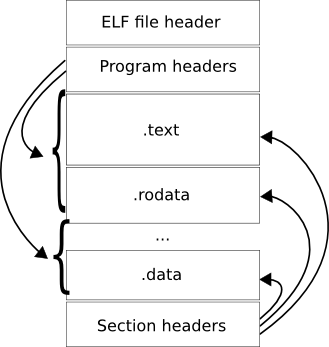
\includegraphics[width=0.5\textwidth]{inc/elf_structure.png}
		\caption{The basic structure of an ELF file. \textit{Image license:} CC BY-SA \cite{elf_structure_orig}}
		\label{elf_structure}
	\end{center}
\end{figure}

All ELF files starts with the four byte identifier \texttt{0x7F}, \texttt{'E'}, \texttt{'L'}, \texttt{'F'} which marks the beginning of the ELF file header. The ELF file header contains general information about a binary, such as its object file type (executable, relocatable or shared object), its assembly architecture (x86-64, ARM, …), the virtual address of its entry point which indicates the starting point of program execution, and the file offsets to the program and section headers.

Each program and section header describes a continuous segment or section of memory respectively. In general segments are used by the linker to load executables into memory with correct access permissions, while sections are used by the compiler to categorize data and instructions. Therefore the program headers are optional for relocatable and shared objects, while the section headers are optional for executables.

\begin{figure}[htbp]
	\begin{center}
		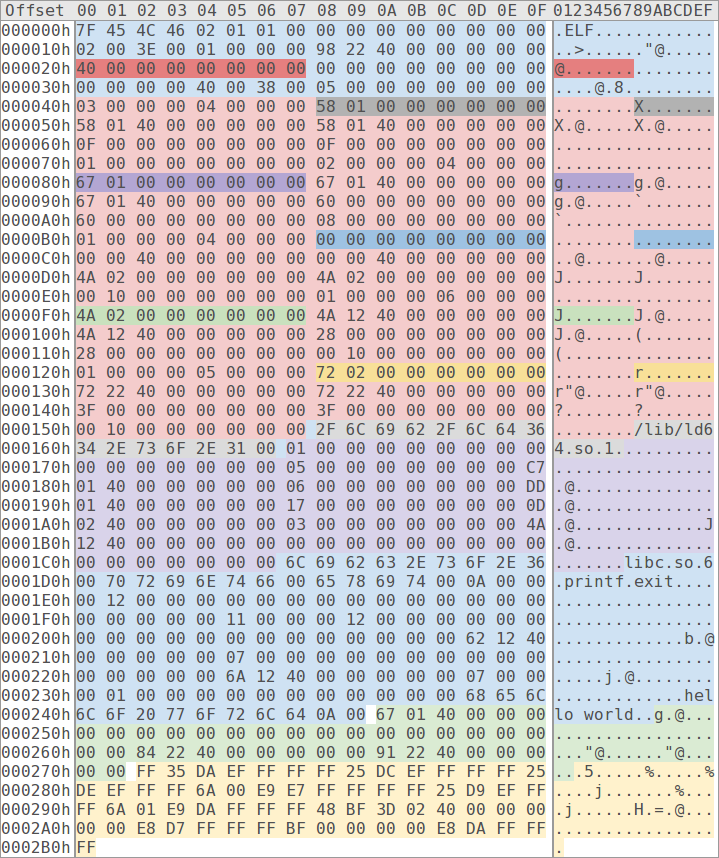
\includegraphics[width=\textwidth]{inc/elf_dissection.png}
		\caption{The entire contents of a simple \textit{``hello world''} ELF executable with color-coded file offsets, sections, segments and program headers, where each file offset is 8 bytes in width and colored using a darker shade of its corresponding segment, section or program header.}
		\label{elf_dissection}
	\end{center}
\end{figure}

To further investigate the structure of ELF files a simple 64-bit \textit{``hello world''} executable has been dissected and its content color-coded. Each file offset of the executable consists of 8 bytes and is denoted in figure \ref{elf_dissection} with a darker shade of the color used by its corresponding target segment, section or program header. Starting at the middle of the ELF file header, at offset \texttt{0x20}, is the file offset (red) to the program table (bright red). The program table contains five program headers which specify the size and file offsets of two sections and three segments, namely the \texttt{.interp} (gray) and the \texttt{.dynamic} (purple) sections, and a \textit{read-only} (blue), a \textit{read-write} (green) and a \textit{read-execute} (yellow) segment.

Several sections are contained within the three segments. The \textit{read-only} segment contains the following sections:

\begin{itemize}
	\item \texttt{.interp}: the interpreter, i.e. the linker
	\item \texttt{.dynamic}: array of dynamic entities
	\item \texttt{.dynstr}: dynamic string table
	\item \texttt{.dynsym}: dynamic symbol table
	\item \texttt{.rela.plt}: relocation entities of the PLT
	\item \texttt{.rodata}: read-only data section
\end{itemize}

The \textit{read-write} segment contains the following section:

\begin{itemize}
	\item \texttt{.got.plt}: Global Offset Table (GOT) of the PLT (henceforth referred to as the GOT as this executable only contains one such table)
\end{itemize}

And the \textit{read-execute} segment contains the following sections:

\begin{itemize}
	\item \texttt{.plt}: Procedure Linkage Table (PLT)
	\item \texttt{.text}: executable code section
\end{itemize}

Seven out of the nine sections contained within the executable are directly related to dynamic linking. The \texttt{.interp} section specifies the linker (in this case \textit{``/lib/ld64.so.1''}) and the \texttt{.dynamic} section an array of dynamic entities containing offsets and virtual addresses to relevant dynamic linking information. In this case the dynamic array specifies that \textit{``libc.so.6''} is a required library, and contains the virtual addresses to the \texttt{.dynstr}, \texttt{.dynsym}, \texttt{.rela.plt} and \texttt{.got.plt} sections. As noted, even a simple \textit{``hello world''} executable requires a large number of sections related to dynamic linking. Further analysis will reveal their relation to each other and describe their usage.

The dynamic string table contains the names of libraries (e.g. \textit{``libc.so.6''}) and identifiers (e.g. \textit{``printf''}) which are required for dynamic linking. Other sections refer to these strings using offsets into \texttt{.dynstr}. The dynamic symbol table declares an array of dynamic symbol entities, each specifying the name (e.g. offset to \textit{``printf''} in \texttt{.dynstr}) and binding information (local or global) of a dynamic symbol. Both the \texttt{.plt} and the \texttt{.rela.plt} sections refers to these dynamic symbols using array indicies. The \texttt{.rela.plt} section specifies the relocation entities of the PLT; more specifically it informs the linker of the virtual address to the \texttt{.printf} and \texttt{.exit} entities in the GOT.

Lets take a step back for a moment and reflect on how dynamic linking is accomplished on a Linux system by reviewing the assembly instructions of the executable \texttt{.text} and \texttt{.plt} sections as outlined in listing \ref{elf_text} and \ref{elf_plt} respectively.

\lstinputlisting[language=nasm,style=nasm,caption={The assembly instructions of the \texttt{.text} section.\label{elf_text}}]{inc/elf_text.asm}

\lstinputlisting[language=nasm,style=nasm,caption={The assembly instructions of the \texttt{.plt} section.\label{elf_plt}}]{inc/elf_plt.asm}

As visualized in listing \ref{elf_text} the first call instruction of the \texttt{.text} section targets the \texttt{.printf} label of the \texttt{.plt} section instead of the actual address of the \textit{printf} function in the \textit{libc} library. The Procedure Linkage Table (PLT) provides a level of indirection between call instructions and actual function (procedure) addresses, and contains one entity per external function as outlined in listing \ref{elf_plt}. The \texttt{.printf} entity of the PLT contains a jump instruction which targets the address stored in the \texttt{.printf} entity of the GOT. Initially this address points to the next instruction, i.e. the instruction denoted by the \texttt{.resolve\_printf} label in the PLT. On the first invokation of \textit{printf} the linker replaces this address with the actual address of the \textit{printf} function in the \textit{libc} library, and any subsequent invokation of \textit{printf} will target the resolved function address directly.

This method of external function resolution is called lazy dynamic linking as it postpones the work and only resolves a function once its actually invoked at runtime. The lazy approach to dynamic linking may improve performance by limiting the number of symbols that require resolution. At the same time the eager approach may benefit latency sensitive applications which cannot afford the cost of dynamic linking at runtime.

A closer look at the instructions denoted by the \texttt{.resolve\_printf} label in listing \ref{elf_plt} reveals how the linker knows which function to resolve. Essentially the \textit{dl\_runtime\_resolve} function is invoked with two arguments, namely the dynamic symbol index of the \textit{printf} function and a pointer to a linked list of nodes, each refering to the \texttt{.dynamic} section of a shared object. Upon termination the linked list of our \textit{``hello world''} process contains a total of four nodes, one for the executable itself and three for its dynamically loaded libraries, namely \textit{linux-vdso.so.1}, \textit{libc.so.6} and \textit{ld64.so.1}.

To summarize, the execution of a dynamically linked executable can roughly be described as follows. Upon execution the kernel parses the program headers of the ELF file, maps each segment to one or more pages in memory with appropriate access permissions, and transfers the control of execution to the linker (\textit{``/lib/ld64.so.1''}) which was loaded in a similar fashion. The linker is responsible for initiating the addresses of the \textit{dl\_runtime\_resolve} function and the aforementioned linked list, both of which are stored in the GOT of the executable. After this setup is complete the linker transfers control to the entry point of the executable, as specified by the ELF file header (in this case the \texttt{.start} label of the \texttt{.text} section). At this point the assembly instructions of the application are executed until termination and external functions are lazily resolved at runtime by the linker through invokations to the \textit{dl\_runtime\_resolve} function.

% --- [ Decompilation Phases ] -------------------------------------------------

\subsection{Decompilation Phases}

A core principle utilized in decompilers is the separation of concern through the use of abstractions, and a lot of work involves translating into and breaking out of various abstraction layers. In general a decompiler is composed of distinct phases which parses, analyzes or transforms the input. These phases are conceptually grouped into three modules to separate concerns regarding source machine language and target programming language. The front-end module parses executable files and translates their platform dependent assembly into a platform independent intermediate representation (IR). The middle-end module performs a set of decompilation passes to lift the IR, from a low-level to a high-level representation, by reconstructing high-level control structures and expressions. Finally the back-end module translates the high-level IR to a specific target programming language. Figure \ref{modules_overview} gives an overview of the decompilation modules and visualizes their relationship.

\begin{figure}[htbp]
	\begin{center}
		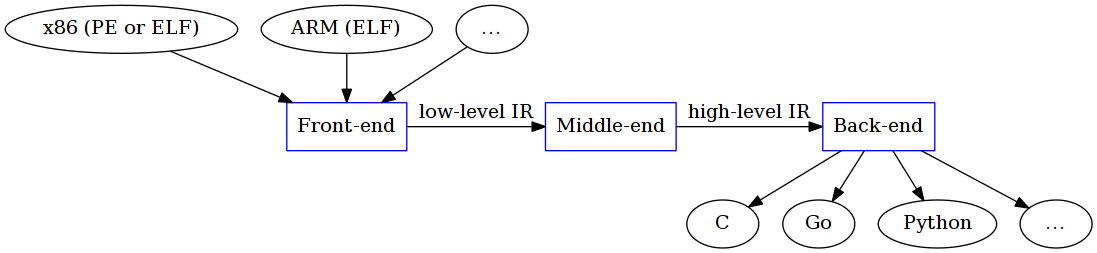
\includegraphics[width=\textwidth]{inc/modules_overview.png}
		\caption{The front-end module accepts several executable file formats (PE, ELF, …) as input and translates their platform dependent assembly (x86, ARM, …) to a low-level IR. The middle-end module then lifts the low-level IR to a high-level IR through a set of decompilation passes. Finally the backend-module translates the high-level IR into one of several target programming languages (C, Go, Python, …).}
		\label{modules_overview}
	\end{center}
\end{figure}

The remainder of this section describes the distinct decompilation phases, most of which have been outlined by Cristina Cifuentes in her influential paper \textit{``Reverse Compilation Techniques''} \cite{rev_comp}.

% ~~~ [ Binary Analysis ] ~~~~~~~~~~~~~~~~~~~~~~~~~~~~~~~~~~~~~~~~~~~~~~~~~~~~~~

\subsubsection{Binary Analysis}

As demonstrated in section \ref{executable_anatomy} parsing even a simple \textit{``hello world''} executable requires extensive knowledge of its binary file format (in this case ELF). The binary analysis phase is responsible for parsing input files of various binary file formats, such as PE and ELF, and present their content in a uniform manner which preserves the relations between file contents, virtual addresses and access permissions. Later stages of the decompilation pipeline builds upon this abstraction to access the file contents of each segment or section without worrying about the underlying file format. Information about external symbols, metadata and the computer architecture of the assembly may also be provided by this abstraction.

% ~~~ [ Disassembly ] ~~~~~~~~~~~~~~~~~~~~~~~~~~~~~~~~~~~~~~~~~~~~~~~~~~~~~~~~~~

\subsubsection{Disassembly}

The disassembly phase (referred to as the syntactic analysis phase in C. Cifuentes paper) is responsible for decoding the raw machine instructions of the executable segments into assembly. At first sight it may seem trivial to implement a disassembler; simply use a lookup table which translates a sequence of bytes to their corresponding assembly instructions.

% TODO: Introduce the various approaches and highlight their individual
% strengths and weaknesses.
%
% NAIVE APPROACH: linear descent disassemblers.
% PROBLEM: Highlight problems with linear descent disassemblers.
%    - rodata (e.g. "hello world") and jump tables in code.
%
% SOLUTION: recursive descent disassemblers.
% PROBLEM: Highlight problems with recursive descent disassemblers.
%    - Distinguish between code and data (e.g. find entry points of functions).
%      Not add functions are directly referred to (e.g. callback functions which
%      are commonly used by GUI applications).
%    - Easy to fool.
%       xor eax, eax
%       cmp eax, 0
%       jz foo+1 ; Cannot disassembly both foo and foo+1.
% foo:
%       add eax, 3
%
% SOLUTION: symbolic execution engines.
% PROBLEM: security, performance, ...?

% ~~~ [ Semantic Analysis ] ~~~~~~~~~~~~~~~~~~~~~~~~~~~~~~~~~~~~~~~~~~~~~~~~~~~~

\subsubsection{Semantic Analysis}

foo

% TODO: Ideoms
%    - 64-bit binops
%    - xor eax, eax ; eax = 0

% ~~~ [ Intermediate Code Generation ] ~~~~~~~~~~~~~~~~~~~~~~~~~~~~~~~~~~~~~~~~~

\subsubsection{Intermediate Code Generation}

foo

% ~~~ [ Control Flow Graph Generation ] ~~~~~~~~~~~~~~~~~~~~~~~~~~~~~~~~~~~~~~~~

\subsubsection{Control Flow Graph Generation}

foo

% ~~~ [ Data Flow Analysis ] ~~~~~~~~~~~~~~~~~~~~~~~~~~~~~~~~~~~~~~~~~~~~~~~~~~~

\subsubsection{Data Flow Analysis}

foo

\cite{type_decomp}

% ~~~ [ Control Flow Analysis ] ~~~~~~~~~~~~~~~~~~~~~~~~~~~~~~~~~~~~~~~~~~~~~~~~

\subsubsection{Control Flow Analysis}

Control-Flow Graph (CFG)

foo

% ~~~ [ Code Generation ] ~~~~~~~~~~~~~~~~~~~~~~~~~~~~~~~~~~~~~~~~~~~~~~~~~~~~~~

\subsubsection{Code Generation}

foo

% --- [ Evaluation of Intermediate Representations ] ---------------------------

\subsection{Evaluation of Intermediate Representations}

% TODO: Very interesting read about the evaluation of IRs specifically for reverse engineering: An Intermediate Representation for Integrating Reverse Engineering Analyses.

% TODO: Check http://indefinitestudies.org/2009/04/03/a-quick-survey-on-intermediate-representations-for-program-analysis/

foo

% ~~~ [ ELIR ] ~~~~~~~~~~~~~~~~~~~~~~~~~~~~~~~~~~~~~~~~~~~~~~~~~~~~~~~~~~~~~~~~~

\subsubsection{ELIR}

% TODO: Research.
% ref: http://www.eresi-project.org/
% Part of ERESI.
% "ERESI development has restarted as of February 2013"
% Seems dead; no new code in 19 months.

foo

% ~~~ [ Hex-Rays Microcode ] ~~~~~~~~~~~~~~~~~~~~~~~~~~~~~~~~~~~~~~~~~~~~~~~~~~~

\subsubsection{Hex-Rays Microcode}

foo

\cite{hexrays}

% ~~~ [ Wire ] ~~~~~~~~~~~~~~~~~~~~~~~~~~~~~~~~~~~~~~~~~~~~~~~~~~~~~~~~~~~~~~~~~

\subsubsection{Wire}

% TODO: Check: Wire - A Formal Intermediate Language for Binary Analysis

foo


% ~~~ [ Valgrind IR ] ~~~~~~~~~~~~~~~~~~~~~~~~~~~~~~~~~~~~~~~~~~~~~~~~~~~~~~~~~~

\subsubsection{Valgrind IR}

foo

% ~~~ [ QEMU IR ] ~~~~~~~~~~~~~~~~~~~~~~~~~~~~~~~~~~~~~~~~~~~~~~~~~~~~~~~~~~~~~~

\subsubsection{QEMU IR}

foo

% ~~~ [ REIL ] ~~~~~~~~~~~~~~~~~~~~~~~~~~~~~~~~~~~~~~~~~~~~~~~~~~~~~~~~~~~~~~~~~

\subsubsection{REIL}

The Reverse Engineering Intermediate Language (REIL) is a very simple and platform independent assembly language. Its instruction set contains only 17 different instructions, each with exactly three (possibly empty) operands. The first two operands are always used for input and the third for output (except for the conditional jump instruction which uses the third operand as the jump target). Furthermore, each instruction has at most one effect on the global state and never any side-effects (such as setting flags) \cite{reil,reil_spec}.

% TODO: Operands have a type, a value and a size.

Thanks to the simplicity of REIL a full definition of its instruction set has been provided in listing \ref{reil_instruction_set}, which includes examples of each instruction and defines their syntax and semantics (in pseudo C-code).

% TODO: Move this listing to an appendix section.
% TODO: Add REIL syntax highlighting.

\lstinputlisting[language=nasm,style=nasm,caption={A full definition of the REIL instruction set. \label{reil_instruction_set}}]{inc/reil_instruction_set.asm}

% TODO: Incorporate notes from "REIL - notes.txt"

The language was originally designed to assist static code analysis and translators from native assembly (x86, PowerPC-32 and ARM-32) to REIL are commercially available. However, the project home page has not been updated since Google acquired zynamics in 2011. Since then approximately 10 papers have been published which references REIL and the adaptation of the language within the open source community seems limited. As of 2015-01-04 only three implementations existed on GitHub (two in Python \cite{barf,pyreil} and one in C \cite{bit}), and the most popular had less than 25 watchers, 80 stars and 15 forks.

% ~~~ [ SAIL ] ~~~~~~~~~~~~~~~~~~~~~~~~~~~~~~~~~~~~~~~~~~~~~~~~~~~~~~~~~~~~~~~~~

\subsubsection{SAIL}

% TODO: Check: SAIL: Static Analysis Intermediate Language with a Two-Level Representation

foo

% ~~~ [ LLVM IR ] ~~~~~~~~~~~~~~~~~~~~~~~~~~~~~~~~~~~~~~~~~~~~~~~~~~~~~~~~~~~~~~

\subsubsection{LLVM IR}

foo

\pagebreak

% === [ Related Work ] =========================================================

\section{Related Work}

foo

% --- [ Native Code to LLVM IR ] -----------------------------------------------

\subsection{Native Code to LLVM IR}

% TODO: Add BAP? Find the project which used QEMU to translate x86 into LLVM IR.

foo

% ~~~ [ Dagger ] ~~~~~~~~~~~~~~~~~~~~~~~~~~~~~~~~~~~~~~~~~~~~~~~~~~~~~~~~~~~~~~~

\subsubsection{Dagger}

foo

% ~~~ [ Fracture ] ~~~~~~~~~~~~~~~~~~~~~~~~~~~~~~~~~~~~~~~~~~~~~~~~~~~~~~~~~~~~~

\subsubsection{Fracture}

foo

% ~~~ [ MC-Semantics ] ~~~~~~~~~~~~~~~~~~~~~~~~~~~~~~~~~~~~~~~~~~~~~~~~~~~~~~~~~

\subsubsection{MC-Semantics}

% TODO: Evaluate and highlight key differences between Dagger, Fracture and McSema.
% Dagger and Fracture rely on TableGen for instruction semantics, McSema does not.

foo

% --- [ Decompilers ] ----------------------------------------------------------

\subsection{Decompilers}

foo

% ~~~ [ dcc ] ~~~~~~~~~~~~~~~~~~~~~~~~~~~~~~~~~~~~~~~~~~~~~~~~~~~~~~~~~~~~~~~~~~

\subsubsection{dcc}

foo

\cite{rev_comp}

% ~~~ [ C-Decompiler ] ~~~~~~~~~~~~~~~~~~~~~~~~~~~~~~~~~~~~~~~~~~~~~~~~~~~~~~~~~

\subsubsection{C-Decompiler}

The \texttt{C-Decompiler} translates machine code into C source code. It focuses primarily on improving the readability of the generated C source code, and does so by extending the traditional decompilation techniques outlined by Cristina Cifuentes in three ways. Firstly, the data flow analysis phase is refined using a shadow stack, which corresponds to a virtual stack capable of tracking stack variables and updates to the stack pointer register. Secondly, the register propagation algorithms are adapted to handle use-def chains across multiple basic blocks. Lastly, library signatures are generated for the C++ Standard Template Library \cite{readable_decomp}.

% ~~~ [ Boomerang ] ~~~~~~~~~~~~~~~~~~~~~~~~~~~~~~~~~~~~~~~~~~~~~~~~~~~~~~~~~~~~

\subsubsection{Boomerang}

foo

\cite{boomerang}

% ~~~ [ Hex-Rays Decompiler ] ~~~~~~~~~~~~~~~~~~~~~~~~~~~~~~~~~~~~~~~~~~~~~~~~~~

\subsubsection{Hex-Rays Decompiler}

foo

\cite{hexrays}

% ~~~ [ The Retargetable Decompiler ] ~~~~~~~~~~~~~~~~~~~~~~~~~~~~~~~~~~~~~~~~~~

\subsubsection{The Retargetable Decompiler}
\label{retargetable_decomp_section}

% TODO: Write about Decompilation as a Services.

foo

\cite{retargetable_decomp}

% ~~~ [ Hopper ] ~~~~~~~~~~~~~~~~~~~~~~~~~~~~~~~~~~~~~~~~~~~~~~~~~~~~~~~~~~~~~~~

\subsubsection{Hopper}

% TODO: Write about the Hopper decompiler. ref: http://www.hopperapp.com/

foo

% --- [ Reverse Engineering Frameworks ] ---------------------------------------

\subsection{Reverse Engineering Frameworks}

foo

% ~~~ [ REcompile ] ~~~~~~~~~~~~~~~~~~~~~~~~~~~~~~~~~~~~~~~~~~~~~~~~~~~~~~~~~~~~

\subsubsection{REcompile}

foo

\cite{recompile}

% ~~~ [ radare ] ~~~~~~~~~~~~~~~~~~~~~~~~~~~~~~~~~~~~~~~~~~~~~~~~~~~~~~~~~~~~~~~

\subsubsection{radare}

foo

\cite{radare}

\pagebreak

%%%%%%%%%%%%%%%%%%%%%%%%%%%%%%%%%%%%%%%%%%%%%%%%%%%%%%%%%%%%%%%%%%%%%%%%%%%%%%%%
% Design and Implementation
%%%%%%%%%%%%%%%%%%%%%%%%%%%%%%%%%%%%%%%%%%%%%%%%%%%%%%%%%%%%%%%%%%%%%%%%%%%%%%%%

% === [ Requirements ] =========================================================

\section{Requirements}

The requirements of each deliverable have been outlined in the succeeding subsections, and are categorized using MoSCoW prioritization \cite{MoSCoW_analysis}; a definition of which is presented in table \ref{MoSCoW_priorities}. Each requirement is directly related to an objective as indicated by the requirements tables of the deliverables. The only objective not covered is objective \ref{obj_data_analysis_library} which was intentionally left as a future ambition.

\begin{table}[htbp]
	\begin{center}
		\begin{tabular}{|l|l|}
			\hline
			Priority & Description \\
			\hline
			MUST & An essential requirement that \textit{must} be satisfied \\
			SHOULD & An important requirement that \textit{should} be satisfied if possible \\
			COULD & A desirable requirement that \textit{could} be satisfied but it is not necessary \\
			WON'T & A future requirement that \textit{will not} be satisfied in this release \\
			\hline
		\end{tabular}
	\end{center}
	\caption{A summary of the MoSCoW (MUST, SHOULD, COULD, WON'T) priorities.}
	\label{MoSCoW_priorities}
\end{table}

% --- [ Literature Review ] ----------------------------------------------------

\subsection{Literature Review}

A top priority of the literature review has been to gain insight into the structural analysis phase (\ref{req_review_structural_analysis}) as the software artefacts heavily depend on it. The other stages of the decompilation pipeline are important to convey the big picture of how components fit together, but the project could still be successful without satisfying \ref{req_review_decomp_stages}.

Several years prior to the initiation of this project the author and his colleges were considering to use LLVM IR for decompilation purposes. In recent years other research groups have started to develop decompilers and reverse engineering components which rely on LLVM IR \cite{decomp_llvm,retargetable_decomp,mcsema}. There may exist an IR which is more suitable in theory, but in practise the collaboration and reuse of others efforts made possible by the vibrant LLVM community is a strong merit in and of itself. The project may therefore be successful even without identifying an optimal IR for decompilation (objective \ref{obj_review_suitable_ir} and \ref{req_review_suitable_ir}).

\begin{table}[htbp]
	\begin{center}
		\begin{tabular}{|l|l|l|l|}
			\hline
			Obj. & Req. & Priority & Description \\
			\hline
			\ref{obj_review_decomp} & \customlabel{req_review_structural_analysis}{\textbf{R1}} & MUST & Describe common structural analysis techniques \\
			\ref{obj_review_decomp} & \customlabel{req_review_decomp_stages}{\textbf{R2}} & SHOULD & Outline the general stages of the decompilation pipeline \\
			\ref{obj_review_suitable_ir} & \customlabel{req_review_suitable_ir}{\textbf{R3}} & COULD & Identify a suitable IR for the decompilation pipeline \\
			\hline
		\end{tabular}
	\end{center}
	\caption{Requirements of the literature review.}
\end{table}

% --- [ LLVM IR Library ] ------------------------------------------------------

\subsection{LLVM IR Library}

The LLVM IR language defines several primitives directly related to code optimization and linking, neither of which convey any useful information for the decompilation pipeline. It is therefore sufficient for this project to support a subset of the LLVM IR language and the relevant requirements should be interpreted as referring to a subset of the language.

The structural analysis tool interacts with other components using LLVM IR. It is therefore required to support reading from and writing to at least one of the representations of LLVM IR. The representations are isomorphic and the standard \texttt{llvm-as} and \texttt{llvm-dis} tools from the LLVM distribution may be used to convert between the assembly language and bitcode representation of LLVM IR. Access to the bitcode representation (\ref{req_ir_library_read_bitcode} and \ref{req_ir_library_write_bitcode}) has therefore been deferred in favour of the assembly language representation (\ref{req_ir_library_read_asm} and \ref{req_ir_library_write_asm}) which has the benefit of being human readable.

The structural analysis library will inspect and manipulate an in-memory representation of LLVM IR (\ref{req_ir_library_mem}) to locate high-level structural patterns and store these findings respectively. Instead of working with sequential lists the structural analysis algorithms will operate on CFGs of basic blocks (\ref{req_ir_library_cfg}). To facilitate the implementation and debugging of these algorithms a visual representation of the CFGs would be beneficial (\ref{req_ir_library_cfg_debug}).

To guarantee the language-agnostic interaction between components, objective \ref{obj_formal_ir} stated that a formal grammar for the LLVM IR had to be located or produced (\ref{req_formal_ir}). Previous efforts have only managed to produce formal grammars for subsets of the LLVM IR language \cite{formal_llvm_ir_spec,formalizing_llvm_ir} and no such grammar has been officially endorsed. The difficult nature of producing a formal grammar only became apparent after discussions with the project supervisor. With this in mind, objective \ref{obj_formal_ir} has been re-evaluated as a future ambition.

\begin{table}[htbp]
	\begin{center}
		\begin{tabular}{|l|l|l|l|}
			\hline
			Obj. & Req. & Priority & Description \\
			\hline
			\ref{obj_ir_library} & \customlabel{req_ir_library_read_asm}{\textbf{R4}} & MUST & Read the assembly language representation of LLVM IR \\
			\ref{obj_ir_library} & \customlabel{req_ir_library_write_asm}{\textbf{R5}} & MUST & Write the assembly language representation of LLVM IR \\
			\ref{obj_ir_library} & \customlabel{req_ir_library_mem}{\textbf{R6}} & MUST & Interact with an in-memory representation of LLVM IR \\
			\ref{obj_ir_library} & \customlabel{req_ir_library_cfg}{\textbf{R7}} & MUST & Produce CFGs from LLVM IR basic blocks \\
			\ref{obj_ir_library} & \customlabel{req_ir_library_cfg_debug}{\textbf{R8}} & COULD & Visualize CFGs using the \texttt{DOT} graph description language \\
			\ref{obj_ir_library} & \customlabel{req_ir_library_read_bitcode}{\textbf{R9}} & WON'T & Read the bitcode representation of LLVM IR \\
			\ref{obj_ir_library} & \customlabel{req_ir_library_write_bitcode}{\textbf{R10}} & WON'T & Write the bitcode representation of LLVM IR \\
			\ref{obj_formal_ir} & \customlabel{req_formal_ir}{\textbf{R11}} & WON'T & Provide a formal grammar of LLVM IR \\
			\hline
		\end{tabular}
	\end{center}
	\caption{Requirements of the LLVM IR library.}
\end{table}

% --- [ Structural Analysis Library ] ------------------------------------------

\subsection{Structural Analysis Library}

A decision was made early on to only support decompilation of compiler generated code from structured high-level languages (\ref{req_structural_analysis_library_reducible_graphs}). Support for arbitrary, unstructured and obfuscated code has been intentionally left out (\ref{req_structural_analysis_library_irreducible_graphs}) to avoid a myriad of special cases.

The structural analysis library must recover the high-level control flow structures of pre-test loops (\ref{req_structural_analysis_library_pre_test_loop}), infinite loops (\ref{req_structural_analysis_library_inf_loop}) and 2-way conditionals (\ref{req_structural_analysis_library_2_way_cond}), as these are found in virtually every high-level language today. Post-test loops (\ref{req_structural_analysis_library_post_test_loop}) and n-way conditionals (\ref{req_structural_analysis_library_n_way_cond}) are also common - but not found in every language (e.g. Python has no \texttt{switch} statements and Go has no \texttt{do-while} loops) - and should therefore be recovered. Support for multi-exit loops (\ref{req_structural_analysis_library_multi_exit_loop}) and nested loops (\ref{req_structural_analysis_library_nested_loop}) could be included if time permits. The recovery of compound boolean expressions is intentionally deferred (\ref{req_structural_analysis_library_compound_bool_expr}) as it would require analysis of instructions within basic blocks in addition to the CFG analysis.

\begin{table}[htbp]
	\begin{center}
		\begin{tabular}{|l|l|l|l|}
			\hline
			Obj. & Req. & Priority & Description \\
			\hline
			\ref{obj_structural_analysis_library} & \customlabel{req_structural_analysis_library_reducible_graphs}{\textbf{R12}} & MUST & Support analysis of reducible graphs \\
			\ref{obj_structural_analysis_library} & \customlabel{req_structural_analysis_library_pre_test_loop}{\textbf{R13}} & MUST & Recover pre-test loops (e.g. \texttt{for}, \texttt{while}) \\
			\ref{obj_structural_analysis_library} & \customlabel{req_structural_analysis_library_inf_loop}{\textbf{R14}} & MUST & Recover infinite loops (e.g. \texttt{while(TRUE)}) \\
			\ref{obj_structural_analysis_library} & \customlabel{req_structural_analysis_library_2_way_cond}{\textbf{R15}} & MUST & Recover 2-way conditionals (e.g. \texttt{if}, \texttt{if-else}) \\
			\ref{obj_structural_analysis_library} & \customlabel{req_structural_analysis_library_post_test_loop}{\textbf{R16}} & SHOULD & Recover post-test loops (e.g. \texttt{do-while}) \\
			\ref{obj_structural_analysis_library} & \customlabel{req_structural_analysis_library_n_way_cond}{\textbf{R17}} & SHOULD & Recover n-way conditionals (e.g. \texttt{switch}) \\
			\ref{obj_structural_analysis_library} & \customlabel{req_structural_analysis_library_multi_exit_loop}{\textbf{R18}} & COULD & Recover multi-exit loops \\
			\ref{obj_structural_analysis_library} & \customlabel{req_structural_analysis_library_nested_loop}{\textbf{R19}} & COULD & Recover nested loops \\
			\ref{obj_structural_analysis_library} & \customlabel{req_structural_analysis_library_irreducible_graphs}{\textbf{R20}} & WON'T & Support analysis of irreducible graphs \\
			\ref{obj_structural_analysis_library} & \customlabel{req_structural_analysis_library_compound_bool_expr}{\textbf{R21}} & WON'T & Recover compound boolean expressions \\
			\hline
		\end{tabular}
	\end{center}
	\caption{Requirements of the structural analysis library.}
\end{table}

% --- [ Structural Analysis Tool ] ---------------------------------------------

\subsection{Structural Analysis Tool}

The primary intention of this project is to create self-contained components which may be used in the decompilation pipelines of other projects. It is therefore of vital importance that the components are able to interact with tools written in other programming languages (\ref{req_structural_analysis_tool_language_agnostic}). The structural analysis tool is one such component which aims to recovers a set of high-level control flow primitives from LLVM IR (\ref{req_structural_analysis_tool_decomp_pass}).

\begin{table}[htbp]
	\begin{center}
		\begin{tabular}{|l|l|l|l|}
			\hline
			Obj. & Req. & Priority & Description \\
			\hline
			\ref{obj_structural_analysis_tool} & \customlabel{req_structural_analysis_tool_decomp_pass}{\textbf{R22}} & MUST & Perform structural decompilation passes on LLVM IR \\
			\ref{obj_structural_analysis_tool} & \customlabel{req_structural_analysis_tool_language_agnostic}{\textbf{R23}} & MUST & Support language-agnostic interaction with other components \\
			\hline
		\end{tabular}
	\end{center}
	\caption{Requirements of the structural analysis tool.}
\end{table}

\pagebreak

% === [ Methodology ] ==========================================================

\section{Methodology}

% TODO: <ask> Should the methodology be written using future, current or past tense?

% TODO: Rewrite to make this section feel right. It is currently too succinct. Elaborate on some topics, and potentially split into multiple sections.

No single methodology will be used for this project, but rather a combination of techniques which have been proven to work well in practice. Continuous Integration will be used throughout the development process to monitor the build status, test cases, and code coverage of each component. The API stability of each component will be governed using Semantic Versioning (vMAJOR.MINOR.PATCH). Prior to version 1.0 the components will be written using either throw-away prototyping or iterative development and the API may change drastically. The implementation correctness will be verified using Test Driven Development where feasible, with test cases written prior to the actual implementation of the API.

% TODO: Explain why this specific methodology was chosen, and justify the methods. The justification may be required to be quite detailed, with in-text references.

% TODO: Add
%    - Attempt to find flaws in the design by stress testing it through proof of concept implementations.
%    - Engage in discussions with the open source community during the design process of any library intended for third party use; specifically the LLVM IR libraries.
%    - Once the design is deemed mature, begin an iterative process of implementation and testing.
%    - Don not be afraid to throw away code and trying new ideas, that is what revision control systems are for!

% TODO: Add
%    - All work was made available on GitHub from day one and the source code was released into the public domain to encourage open source adaptation and interaction.

% --- [ Evolutionary Development and Throwaway Prototyping ] -------------------

\subsection{Evolutionary Development and Throwaway Prototyping}

foo

% ~~~ [ Revision Control System ] ~~~~~~~~~~~~~~~~~~~~~~~~~~~~~~~~~~~~~~~~~~~~~~

\subsubsection{Revision Control System}

foo

% --- [ Public Issue Tracking ] ------------------------------------------------

\subsection{Public Issue Tracking}

% TODO: Add
%    - The project plan will be organized using the GitHub issue tracker, where each issue corresponds to a task. Milestones, containing a set of issues, will track the progress of the project and enforce deadlines.
%    - To facilitate time management each task will be tracked using the GitHub issue tracker, and larger tasks will be divided into suitably sized sub-tasks. The smaller sub-tasks help maintain focus and make it easier to establish reasonable deadlines.

% TODO: Add project plan?
%    - The project plan will be managed using the GitHub issue tracker, and actively maintained throughout the project. Each task (research topic, unresolved problem, software feature, etc) will be allocated a dedicated issue tracking its progress. The issues include relevant discussions of identified risks, potential problems and proposed solutions. The project plan provides an overview of the active issues, using milestones to group issues and assign deadlines.

foo

% --- [ Test Driven Development ] ----------------------------------------------

\subsection{Test Driven Development}

foo

\pagebreak

% === [ Design ] ===============================================================

\section{Design}

% TODO: Add design notes
%    - The LLVM IR libraries are developed as reusable components for compilers, decompilers, and other semantic analysis tools. They aim to support generic semantic analysis applications, while satisfying the explicit requirements [1] of the third party llgo compiler.
%
% [1]: https://github.com/go-llvm/llvm/issues/40

% TODO: Add
%   - A decompilation system composed of individual components and based on the principle of separation of concerns.
%   - The system must be language-agnostic so that decompilation passes can be reused from other programming language environments.

foo

% --- [ Choice of Programming Language ] ---------------------------------------

\subsection{Choice of Programming Language}

% TODO: Clarify the benefits and drawbacks of using Go over C++ which would be the obvious choice for LLVM IR heavy projects. Choosing not to use C++ validates the language-agnostic aspects of the design.
% - Compilation speed. ll2dot takes > 1.5m whereas a regular Go program takes < 1s.

% TODO: Mention software composition.

% TODO: Add and tie in to the pragmatic aspects of Go?
%    * tooling?
%       - "go get" can locate all dependencies.
%       - compilation time is linear rather than exponential with regards to dependencies.
%    * automation?

foo

% --- [ Decompiler Pipeline ] --------------------------------------------------

\subsection{Decompiler Pipeline}

% TODO: Describe where the "restructure" component fits in the overall decompilation pipeline. Mention which projects and tools that may be used to fill the gaps. bin_descend and IDA python script of MC-Semantics -> Google Protocol Buffer -> cfg_to_bc -> LLVM IR

% TODO: Rewrite and clarify.

The decompilation pipeline is made of up several components which are conceptually grouped into three modules. The front-end module translates a variety of inputs (such as binary files and source code) into LLVM IR by utilizing a collection of tools developed by several independent open source projects. The middle-end lifts the LLVM IR to a high-level representation by conducting a control flow analysis which generates a structured CFG of each function. The back-end generates high-level control-flow primitives such as if-statements and for-loops based on the structured CFG. In addition it translates the individual instructions of the LLVM IR to expressions and statements of the target programming language (in this case Go). The interaction between the front-end, middle-end and back-end modules is visualized in figure \ref{decompilation_pipeline}.

% * Front-end
%    - binary -> LLVM IR ([MC-Semantics](https://github.com/trailofbits/mcsema), [Dagger](http://dagger.repzret.org/) or [Fracture](https://github.com/draperlaboratory/fracture))
%    - source code -> LLVM IR (clang, ghc, rustc, ...)
% * Middle-end
%    - LLVM IR -> Unstructured CFG ([ll2dot](https://github.com/mewrev/ll2dot))
%    - Unstructured CFG -> Structured CFG ([iso](https://github.com/mewrev/graphs) and [merge](https://github.com/mewrev/graphs).)
%       + Truthfully `ll2go` doesn't make direct use of `iso` or `merge` but rather the graph libraries. A future ambition is to allow `iso` and `merge` to output JSON such that they may be used directly by `ll2go`.
% * Back-end
%    - Structured CFG -> Go ([ll2go](https://github.com/mewrev/ll2go))


\begin{figure}[htbp]
	\begin{center}
		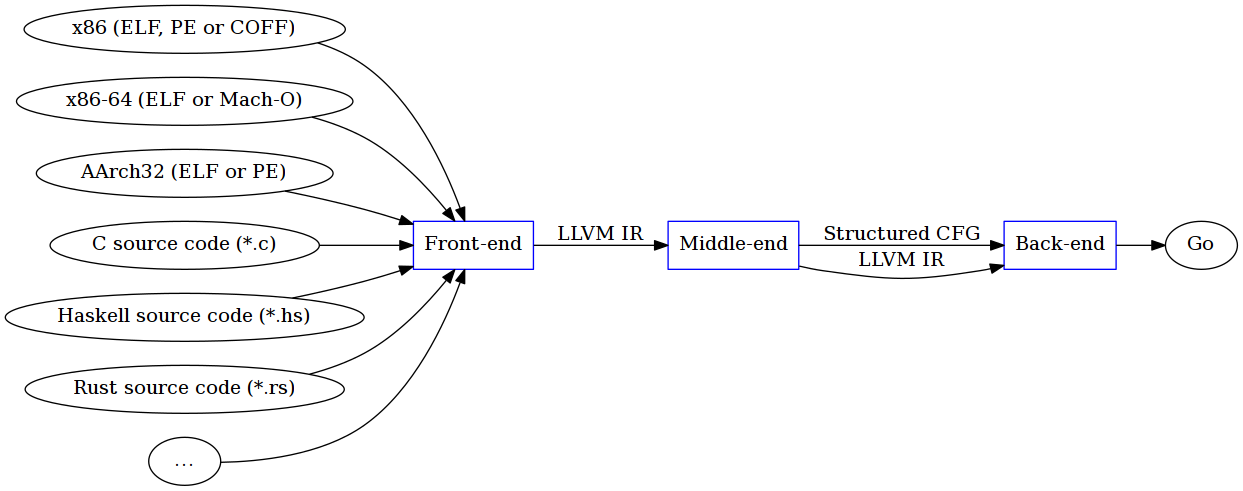
\includegraphics[width=\textwidth]{inc/decompilation_pipeline.png}
		\caption{foo}
		\label{decompilation_pipeline}
	\end{center}
\end{figure}


\subsubsection{Front-end}

% TODO: Rewrite and clarify.

The front-end module is responsible for converting the input into LLVM IR. Two common scenarios exists, converting binary files (e.g. executables, shared libraries and relocatable object code) and converting source code (e.g. C, Haskell, Rust, …) into LLVM IR. The first scenario is presented in figure \ref{binary_to_llvm} and the second in figure \ref{source_to_llvm}.

% TODO: Mention opt --mem2reg.

\begin{figure}[htbp]
	\begin{center}
		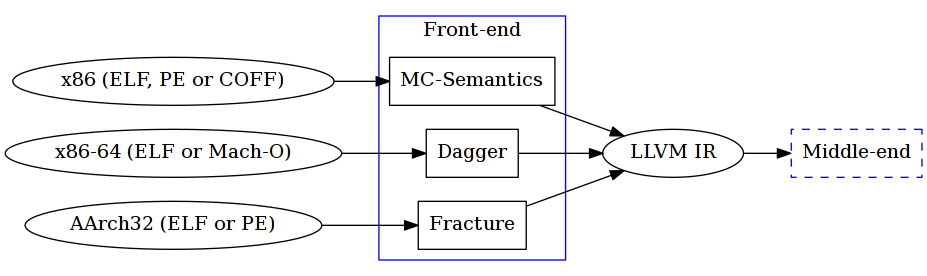
\includegraphics[width=\textwidth]{inc/front-end_binary.png}
		\caption{foo}
		\label{binary_to_llvm}
	\end{center}
\end{figure}

\begin{figure}[htbp]
	\begin{center}
		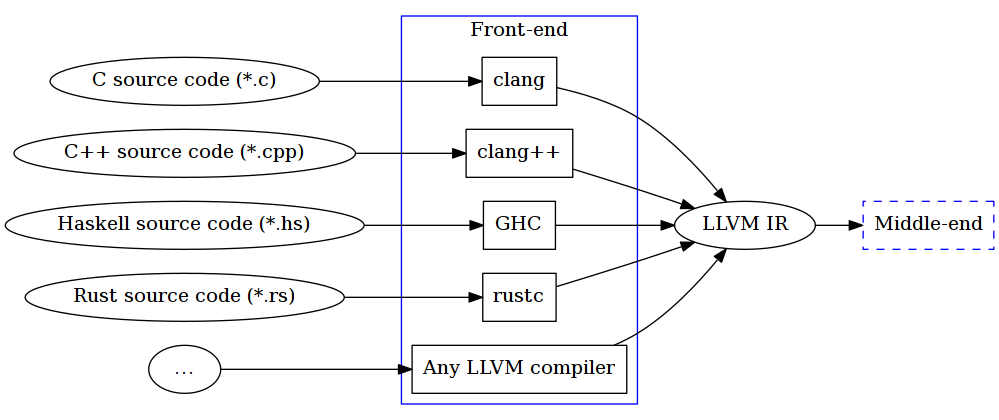
\includegraphics[width=\textwidth]{inc/front-end_source.png}
		\caption{foo}
		\label{source_to_llvm}
	\end{center}
\end{figure}

\subsubsection{Middle-end}

% TODO: Rewrite and clarify.

% TODO: Create a restructure tool which replaces the use of iso.

The middle-end is responsible for lifting the LLVM IR to a high-level representation through a series of decompilation passes. The \texttt{ll2dot} tool generates a CFG (in the DOT file format) for each function of a given LLVM IR input file. The \texttt{iso} tool searches for subgraph isomorphisms of control flow primitives in a given CFG. Once located the nodes identified subgraph are merged into a single node which is labeled with the high-level control flow primitive. Successive iterations continue to simplify the CFG until only one node is left, at which point the high-level control flow structure has been recovered. Should the \texttt{iso} tool fail to reduce the graph into a single node, the graph is considered irreducible with regards to the supported high-level control-flow primitives. The interaction between the front-end, the \texttt{ll2dot} and \texttt{iso} tools of the middle-end and the back-end is illustrated in figure \ref{middle_end}.

\begin{figure}[htbp]
	\begin{center}
		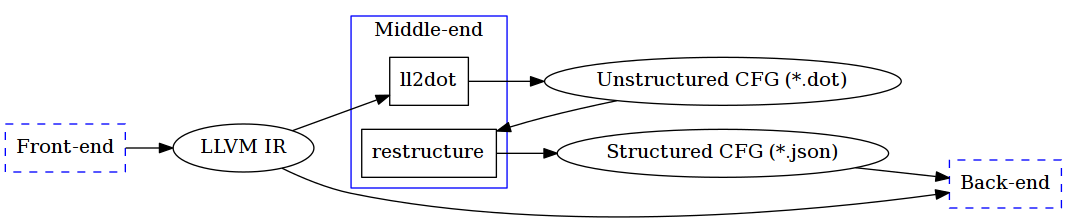
\includegraphics[width=\textwidth]{inc/middle-end.png}
		\caption{foo}
		\label{middle_end}
	\end{center}
\end{figure}

\subsubsection{Back-end}

% TODO: Rewrite and clarify.

% TODO: Add ref to rsc's grind tool.

% TODO: Proof-of-concept. Implement a back-end for another language and written in another language. This would stress test the language-agnostic aspects of the design, thus making sure that the heavy-lifting is done in the middle-end and not in ll2go.

The back-end is responsible for translating the structured control-flow graph of the LLVM IR into a target programming language. The \texttt{ll2go} tool is a proof of concept back-end which produces unpolished Go source code. The polishing is done by separate tools which fixes potential compilation issues and makes the code more idiomatic. The interaction between the middle-end and the back-end is illustrated in figure \ref{back_end}. Currently the \texttt{ll2gofix} replaces return-statements in the \texttt{main} function with calls to \texttt{os.Exit}, which is required since the \texttt{main} function has no return arguments in Go. Instead the Go runtime calls \texttt{os.Exit} with the status-code \texttt{0} once \texttt{main} returns to signal successful termination. This eliminates the need to always end the \texttt{main} function with a \texttt{return 0;} statement as is common practise in C. A future ambition is to make use of and possibly contribute to the \texttt{grind} tool which moves variable declarations closer to their usage, and thus improving readability of the code. Generally the aim is to keep the \texttt{ll2go} tool as simple as possible. The middle-end is responsible for the structural analysis, and as a future ambition the data flow analysis. Since the complexity of the back-end is kept to a minimum it should be trivial to implement support for other output languages.

\begin{figure}[htbp]
	\begin{center}
		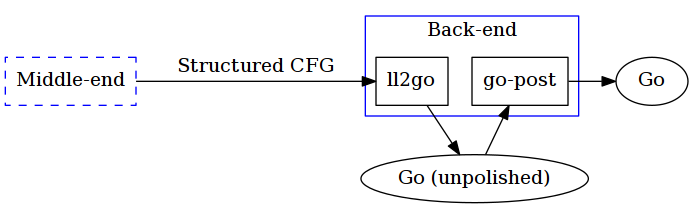
\includegraphics[width=\textwidth]{inc/back-end.png}
		\caption{foo}
		\label{back_end}
	\end{center}
\end{figure}

% --- [ System Architecture ] --------------------------------------------------

\subsection{System Architecture}

% TODO: Visualize the dependency graph of the "restructure" tool and describe in detail what input it expects and what output it produces.

% TODO: Write about. Input and output LLVM IR to operate well with components written in other languages. Output LLVM IR with information about high-level control structures stored in the basic block names or in metadata.

foo

% TODO: Mention package division.

\subsection{Data-driven Design}

% TODO: Add notes about the use of DOT-files to describe control-flow primitives. Think if and how this could be pushed further to facilitate the development of future back-ends.

\subsection{Limitations}

% TODO: Add limitations related to the design choices. Which limitations are easily solvable given more time and which are fundamentally part of the design.
%    - No support for n-way conditionals (e.g.switch-statements).

foo

% --- [ Security Assessment ] --------------------------------------------------

\subsection{Security Assessment}

To assess the security of the decompiler pipeline, lets imagine a scenario in which users are given access to the implementation details and source code of the entire system and may provide arbitrary input to any of its components. A potential scenario could involve a web site which provides decompilation as a service and allows its users to interact with the various stages of the decompiler pipeline. The Retargetable Decompiler (see section \ref{retargetable_decomp_section}) provides such a service, except it only allows users to interact with the binary analysis stage of the pipeline and its source code is proprietary. The scope of this security assessment will be limited to the various components of the decompiler pipeline and their interaction. In particular security issues related to the operating system, network stack, web server and web page (e.g. SQL-injection and XSS vulnerabilities) of the decompilation service are intentionally excluded from the scope of the security assessment.

The objective of an attacker may be to escalate their privileges in a system by exploiting it to execute actions not intended by design. Since the security of any system is only as strong as its weakest link, it is critical to identify and isolate likely targets for attacks. Projects which consist of or depend on large C or C++ code bases may exhibit memory safety issues, such as buffer overflows or use-after-free vulnerabilities. These issues are considered low-hanging fruit for attackers and have a long history of successful exploitation \cite{for_fun_and_profit}. Several modern programming languages (including Go) provide memory safety guarantees and may solve these issues by inserting bounds-checking for array accesses and using garbage collection for memory management. Code written in memory safe languages may still contain other security vulnerabilities caused by logic errors or insufficient validation, sanitation and parametrization of input (e.g. command injection and directory traversal vulnerabilities).

The number of lines of code in a project may give an indication to the project's complexity and to some extent its potential attack surface. As summarized in table \ref{loc_summary} every component of the decompiler pipeline except \texttt{iso} depends on LLVM. The LLVM code base contains approximately \numprint{800000} lines of C++ source code, and even if only a portion of the code will be linked into the executables it is an interesting target for attacks. One thing to keep in mind is that there are several high-end users of the LLVM project (such as Apple, Intel, NVIDIA and Sony \cite{llvm_users}) and it has a well established code reviewing process. Some of the LLVM developers are also very well educated in common security vulnerabilities and have developed the Clang Static Analyzer, which is a static source code analysis that locates bugs (such as buffer overflows and use-after-free issues) in C and C++ programs \cite{clang_analyzer}. The LLVM project may contain several security issues due to its size, but they are most likely difficult to discover since the low-hanging fruit have been caught by the Clang Static Analyzer.

\begin{table}[htbp]
	\begin{center}
		\begin{tabular}{|l|l|l|l|}
			\hline
			\textbf{Project} & \textbf{Language} & \textbf{Lines} & \textbf{Dependencies} \\
			\hline
			\multicolumn{4}{|l|}{\hspace{4ex} \textit{Front-end}} \\
			\hline
			Dagger & C++ & \numprint{2000} & LLVM \\
			Fracture & C++ & \numprint{20000} & LLVM \\
			MC-Semantics & C++ & \numprint{25000} & LLVM and Google Protocol Buffers \\
			\hline
			\multicolumn{4}{|l|}{\hspace{4ex} \textit{Middle-end}} \\
			\hline
			ll2dot & Go & \numprint{500} & LLVM and dot \\
			iso & Go & \numprint{2000} & dot \\
			\hline
			\multicolumn{4}{|l|}{\hspace{4ex} \textit{Back-end}} \\
			\hline
			ll2go & Go & \numprint{1500} & LLVM, llvm (Go), iso and dot \\
			\hline
			\multicolumn{4}{|l|}{\hspace{4ex} \textit{Dependencies}} \\
			\hline
			LLVM & C++ & \numprint{800000} & - \\
			Google Protocol Buffers & C++ & \numprint{125000} & - \\
			llvm (Go) & Go & \numprint{5000} & - \\
			dot & Go & \numprint{7000} & - \\
			\hline
		\end{tabular}
	\end{center}
	\caption{A rough summary of each project specifying their programming language, number of lines of code and dependencies.}
	\label{loc_summary}
\end{table}

\pagebreak

% === [ Development ] ==========================================================

\section{Development}

% TODO: Brainstorm about which sections are actually relevant and how they should be structured.

% TODO: Mention the following trivias:
%    - Identify unused tokens (hash and backspace) in the C++ code base and submit a patch which was commited to remove these. (http://reviews.llvm.org/D7248)
%    - Discuss API design with members of the open source community.
%    - Ask experienced LLVM developers of insight into possible inconsistencies with LLVM IR. Some highlighted inconsistent behaviour and some were intended behaviour. (LLVM-dev mailing list)

% Hints for Computer System Design (1983) - Butler Lampson
%    "Handle normal and worst case seperately"

foo

% --- [ LLVM IR Library ] ------------------------------------------------------

\subsection{LLVM IR Library}

foo

% --- [ Control Flow Graph Generation Tool ] -----------------------------------

\subsection{Control Flow Graph Generation Tool}

foo

% --- [ Subgraph Isomorphism Search Algorithm ] --------------------------------

\subsection{Subgraph Isomorphism Search Algorithm}

Implementing the subgraph isomorphism search algorithm was without doubt the most difficult endeavour of the entire project. It took roughly five iterations of implementing, evaluating and rethinking the algorithm to find an approach which felt right and another two iterations to develop a working implementation which passed all the test cases.

% TODO: Incorporate notes from iso_algorithm_notes.txt.

% --- [ Control Flow Analysis Tool ] -------------------------------------------

\subsection{Control Flow Analysis Tool}

foo

% --- [ Decompiler Back-end Tool ] ---------------------------------------------

\subsection{Decompiler Back-end Tool}

foo

% --- [ Idiomatic Coding ] -----------------------------------------------------

\subsection{Idiomatic Coding}

Making effective use of a programming language requires more than simply learning its syntax and key features. With a reasonable understanding of the underlying design decisions behind a programming language and the historic factors which drove its development one may infer the governing principles and key beliefs of its developers. These principles and beliefs influence every aspect of the software development process; they determine how programs are structured and how problems are solved. One of the primary driving forces behind the development of the Go programming language is pragmatism, the idea of which was captured in the following quote by Samuel Tesla shortly after Go was released in 2009:

\begin{quote}
	\textit{``Go is not meant to innovate programming theory. It's meant to innovate programming practice.''} - Samuel Tesla, Dec 2009 \cite{pragmatic}
\end{quote}

In 2012 Rob Pike (one of the Go language inventors) gave a talk titled \textit{``Less is exponentially more''} which included a personal description of the historic events leading up to the inception of Go. The starting point of the language was C, not C++, which Go aimed to simplify further by removing cruft. This stands in direct contrast to the direction of C++ which gains more features with each passing release. The \textit{less is more} mindset is deeply rooted in the mentality of Go developers and there is a strong emphasis on the use of composition to solve problems.

\begin{quote}
	\itshape
	``If C++ and Java are about type hierarchies and the taxonomy of types, Go is about composition.

	Doug McIlroy, the eventual inventor of Unix pipes, wrote in 1964 (!):

	\begin{quote}
		We should have some ways of coupling programs like garden hose--screw in another segment when it becomes necessary to massage data in another way. This is the way of IO also.
	\end{quote}

	That is the way of Go also. Go takes that idea and pushes it very far. It is a language of composition and coupling.''
	\normalfont
	- Rob Pike, 2012 \cite{less_is_more}
\end{quote}

Every aspect of Go development embodies the UNIX philosophy (see figure \ref{unix_philosophy}) which comes as no surprise since Ken Thompson (one of the original inventors of UNIX) is part of the core Go team.

\begin{figure}[htbp]
	\begin{center}
		\begin{quote}
			\textit{``Write programs that do one thing and do it well. Write programs to work together.''} \cite{art_of_unix}
		\end{quote}
		\caption{The UNIX philosophy.}
		\label{unix_philosophy}
	\end{center}
\end{figure}

% --- [ Documentation ] --------------------------------------------------------

\subsection{Documentation}

% TODO: Add example use cases (perhaps also covering related projects such as McSema)?

A set of source code analysis tools are used to automate the generation and presentation of documentation. The main benefit of this approach is that only one version of the documentation has to be maintained and it is kept within the source code, thus preventing it from falling out of sync with the implementation. UNIX manual pages are generated for command line tools using \texttt{mango} \cite{mango}, which locates the relevant comments and command line flag definitions in the source code. Library documentation is presented using \texttt{godoc} \cite{godoc} (a tool similar to \texttt{doxygen}), and may be accessed through a web or command line interface.

The GoDoc.org server hosts an instance of \texttt{godoc} which presents the documentation of publicly available source code repositories. An online version of the documentation has been made available for each artefact using this service.

\begin{itemize}
	\item Library for interacting with LLVM IR (\textit{work in progress}) \\ \url{https://godoc.org/github.com/mewlang/llvm}
	\item LLVM IR Control Flow Graph generation tool \\ \url{https://godoc.org/github.com/mewrev/ll2dot}
	\item Subgraph isomorphism search algorithms for reconstructing high-level control flow primitives and related tools \\ \url{https://godoc.org/github.com/mewrev/graphs}
	\item Decompiler back-end tool (\textit{proof of concept}) \\ \url{https://godoc.org/github.com/mewrev/ll2go}
\end{itemize}

% --- [ Verification ] ---------------------------------------------------------

\subsection{Verification}

\subsubsection{Test Cases}

% TODO: Add
%    - Use the Clang compiler to produce test cases, as it is capable of emitting LLVM IR from C source code. The goal will be to reconstruct the high- level control flow structures (such as for- loops, if-else statements, etc) of the original C code from the LLVM IR.

While developing the lexer for the LLVM IR assembly language

foo

\subsubsection{Code Coverage}

\ref{iso_code_coverage}

\begin{figure}[htbp]
	\begin{center}
		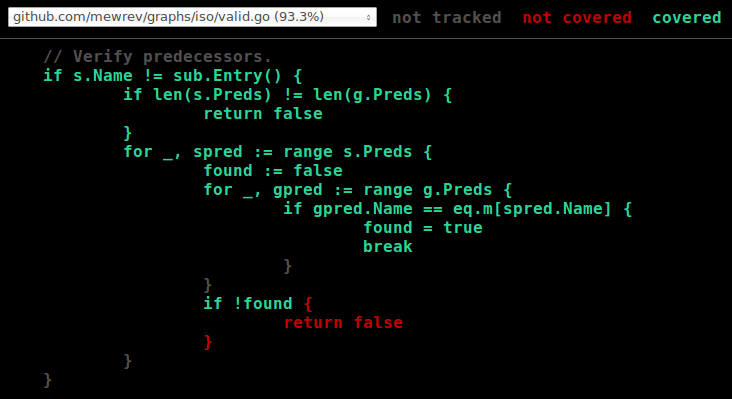
\includegraphics[width=\textwidth]{inc/iso_code_coverage.png}
		\caption{Extract from the code coverage of the subgraph isomorphism search algorithm.}
		\label{iso_code_coverage}
	\end{center}
\end{figure}

foo

% --- [ Optimization ] ---------------------------------------------------------

\subsection{Optimization}

foo

\subsubsection{Benchmarks}

percentage delta.

\texttt{benchcmp}

foo

\subsubsection{Profiling}

% TODO: Add bottle neck example
%    inc/lexer_pprof_before.svg

% TODO:
%    - CPU profiling
%       go test -cpuprofile=a.out
%    - Memory profiling
%       go test -memprofile=a.out

\texttt{go tool pprof}

foo

% --- [ Continuous Integration ] -----------------------------------------------

\subsection{Continuous Integration}

The Continuous Integration (CI) practise originated from the Extreme Programming methodology \cite{xp} but has reached a much broader audience in recent years. Today most large scale software projects rely on CI server farms which continuously compile and test new versions of the source code.

This project makes use of Travis CI, which is tightly integrated with GitHub, to run a series of automated tests for each commit to the source code repository. The tests are varied and range from identifying source code formatting and coding style issues to monitoring the build status and test coverage. A future ambition is to run benchmarks for each commit to quickly identify performance regressions.

\subsubsection{Source Code Formatting}

Instead of relying on a formatting style guide the Go project enforces a single formatting style using \texttt{gofmt} (a tool similar to \texttt{indent}) which automatically formats Go source code. The adoption of this tool is widespread within the Go community as indicated by a survey conducted back in 2013. The survey found that 70\% of the publicly available Go packages were formatted according to the rules of \texttt{gofmt} \cite{gofmt_70percent}, a figure which is likely to have increased since then.

Using a single formatting style for all Go source code may at first seem like a small deal, but the advantages are vast. It becomes easier to write code as one may focus on the problem at hand rather than minor formatting issues. Similarly it becomes easier to read code when it is formatted in a familiar and uniform manner. We may focus our entire attention at understanding the semantics of the code without being distracted by inconsistent or unfamiliar formatting. And perhaps most importantly, it prevents useless discussions about which formatting style is the right one.

Several text editors supports adding pre-save hooks which executes a command to pre-process the text before saving it. This mechanism may be used with the \texttt{godoc} tool to automatically enforce its formatting style each time a source file is saved. One of the CI tests catches and reports incorrectly formatted source code, should a programmer forget to install such a hook.

\subsubsection{Coding Style}

\texttt{golint}

foo

\subsubsection{Code Correctness}

\texttt{go vet}

foo

\subsubsection{Build Status}

\texttt{go get}

foo

\subsubsection{Test Cases}

\texttt{go test}

foo

\subsubsection{Code Coverage}

\texttt{go test -cover}

foo

\subsubsection{Data Race Detection}

\texttt{go test -race}

foo

\pagebreak

%%%%%%%%%%%%%%%%%%%%%%%%%%%%%%%%%%%%%%%%%%%%%%%%%%%%%%%%%%%%%%%%%%%%%%%%%%%%%%%%
% Evaluation and Conclusion
%%%%%%%%%%%%%%%%%%%%%%%%%%%%%%%%%%%%%%%%%%%%%%%%%%%%%%%%%%%%%%%%%%%%%%%%%%%%%%%%

% === [ Evaluation ] ===========================================================

\section{Evaluation}

foo

% --- [ Evaluation against Requirements ] --------------------------------------

\subsection{Evaluation against Requirements}

foo

% --- [ TODO ] -----------------------------------------------------------------

\subsection{TODO}

foo

% --- [ Profiling and Benchmarks ] ---------------------------------------------

\subsection{Profiling and Benchmarks}

foo

\pagebreak

% === [ Future Work ] ==========================================================

\section{Future Work}

% TODO: Add notes from IDEAS.txt.
%    - grind

% * Finish developing the LLVM IR library and replace the C++ binding with a pure Go implementation. This should decrese build times significantly and simplify the overall complexity of the project by several orders of magnitude.

% * Formal Grammar for a subset of LLVM IR
%    - Mention previous (partial but incomplete) work.

% * Third Party Adaptation

% * Data Flow Analysis.

% * Stress test the design by implementing another back-end written in and for another programming language.

% TODO: Fuzz the LLVM IR parser by generating valid LLVM from the EBNF grammar (similar to gosmith).

foo

\pagebreak

% === [ Conclusion ] ===========================================================

\section{Conclusion}

This section concludes the project report and includes subjective reflections from the author. For the remainder of this section I will switch to a first person narrative.

% --- [ Project Summary ] ------------------------------------------------------

\subsection{Project Summary}

% TODO: Summarise the key findings of your report. No new information should be included.

foo

% --- [ Personal Development ] -------------------------------------------------

\subsection{Personal Development}

This is the largest project I have undertaken in my life and I feel satisfied with the outcome and proud of what I have been able to accomplished. It has re-enforced my belief that any problem is solvable when broken into smaller subproblems and instilled me with a feeling that anything is possible. The project has allowed me to mature as a software developer and I now feel more confident in utilizing best practies such as TDD, CI and semantic versioning. I have also matured as a developer and gained experience with implementing a semi-large project and structuring it into several smaller self-contained projects.

% --- [ Final Thoughts ] -------------------------------------------------------

\subsection{Final Thoughts}

My happiest moment during the project was when the larger components started working and could be connected to form a complete system. It feels great having started out with a vague idea of how the decompiler could work, gradually gaining new insights and refining its design after researching and building on the knowledge of others, developing and iteratively reimplementing the various components until they feel just right, finally arriving at a working prototype and seeing the full system in action! If there is one key idea I want to leave you with it is that the composition of independent components, each with a single purpose and well-defined input and output, is a powerful concept for solving complex problems.

\pagebreak

%%%%%%%%%%%%%%%%%%%%%%%%%%%%%%%%%%%%%%%%%%%%%%%%%%%%%%%%%%%%%%%%%%%%%%%%%%%%%%%%
% References
%%%%%%%%%%%%%%%%%%%%%%%%%%%%%%%%%%%%%%%%%%%%%%%%%%%%%%%%%%%%%%%%%%%%%%%%%%%%%%%%

% === [ References ] ===========================================================

\section{References}

\renewcommand{\refname}{\vskip -1cm}
\bibliography{references}

\end{document}
